% chapters/cap4_metod/cap4.tex

\chapter{Metodología}
\label{cap:metodologia}

En este capítulo se describe de manera detallada la metodología aplicada para la resolución de la ecuación de advección unidimensional para dos partículas SPH. A partir de la base teórica establecida, se detalla el modelado del problema y la transición hacia las caminatas cuánticas de tiempo continuo y las consideraciones físicas necesarias para su implementación.

\section{Análisis del trabajo previo}

Es fundamental resaltar el trabajo previo realizado en \cite{auyeung2024, auyeung2025}, el cual establece las bases teóricas de \emph{Quantum SPH} (QSPH). En su investigación, se realiza de forma detallada la formulación matemática que traduce la dinámica clásica de partículas SPH \eqref{eq:sph_advection_discrete}, a un formalismo válido dentro de la mecánica cuántica. Siguiendo este trabajo, la formulación a la que se llega para ver el paso del tiempo de la cantidad advectada $u$ en la partícula $j$ está dada por:

\begin{equation}
    u_j(t_0 + \Delta t) = u_j(t_0) - c \Delta t \, v N |\mathbf{a}| \Re(\langle a | \nabla_j W_{jk} \rangle)
    \label{eq:auyeung}
\end{equation}

Esta ecuación demuestra que es posible alcanzar estados válidos que representan la dinámica del fluido, por medio de QSPH, en un computador cuántico. Partiendo de esta base, y asumiendo por simplicidad una separación espacial uniforme entre las partículas ($\Delta x_k = \Delta x$) para un paso de tiempo constante $\Delta t$, en \cite{auyeung2025} reescriben la ecuación de advección SPH de la siguiente manera:

\begin{equation}
    u_j(t_0+1) = u_j(t_0) - c N \Delta x \sum_{k \neq j} V_{jk} + c N \Delta x \sum_{k \neq j} u_k(t_0) V_{jk}
    \label{eq:auyeung_14}
\end{equation}

donde $V_{jk} = \nabla_j W_{jk}/(vN) + ib_{jk} $ y $v = \max|\nabla_j W_{jk}|$. De esta forma se encapsula la evaluación del kernel de suavizado junto con los términos de normalización imaginarios necesarios para garantizar la unitariedad en el computador cuántico. Para adaptar esta expresión al formalismo de las caminatas cuánticas continuas (CTQW), los autores definen las amplitudes de probabilidad, equivalentes a los coeficientes de evolución temporal. La amplitud de autointeracción para la partícula $j$ se define como:

\begin{equation}
    \alpha_{jj} = 1 + c N \Delta x \Re(\sum_{k \neq j} V_{jk})
    \label{eq:auyeung_15}
\end{equation}

mientras que la amplitud de interacción que gobierna el flujo desde las partículas vecinas $k$ hacia $j$ está dada por:

\begin{equation}
  \alpha_{jk} = -c N \Delta x \Re(V_{jk})
    \label{eq:auyeung_16}
\end{equation}

Sustituyendo estas amplitudes en la ecuación \eqref{eq:auyeung_14}, se llega a la forma compacta de la actualización temporal que dicta cómo evoluciona la cantidad advectada $u_j$:

\begin{equation}
    u_j(t_0+1) = \alpha_{jj} u_j(t_0) + \sum_{k} \alpha_{kj} u_k(t_0)
    \label{eq:auyeung_17}
\end{equation}

Esta formulación define valores de una matriz de evolución temporal a través de la formación de los coeficientes $\alpha_{jj}$ \eqref{eq:auyeung_15}, $\alpha_{jk}$ \eqref{eq:auyeung_16}, en los cuales lleva consigo toda la información del escenario y la interacción con cada partícula.

No obstante, la formulación alcanzada en dichos trabajos no representa un SPH puro en su concepción lagrangiana. Debido a la formulación QSPH \eqref{eq:auyeung}, las partículas no se encuentran libres; en su lugar, se asume un $\Delta x$ constante que no varía con el tiempo ni con la interacción. Las partículas permanecen fijas en un espacio definido. Aunque los autores reconocen esta limitación, este paradigma nos motiva a replantear el problema desde la naturaleza de un CTQW. Ese anclaje de posiciones es también el de este TFM y explica que el dímero tenga una relajación en lugar de advectar un perfil.


\section{Analogía con CTQW}
\label{subsec: analogía}

En la exploración de grafos mediante CTQW, los nodos permanecen fijos en el espacio y no dependen estrictamente de los nodos circundantes para definir su posición. Sin embargo, la información que fluye a través del grafo, su amplitud de probabilidad, sí depende de la topología local (sus vecinos y el escenario general). Esta dinámica exhibe un paralelismo profundo con una malla euleriana o un escenario SPH predefinido, donde dejamos que la ``información'' (el fluido) se propague a través de los nodos estáticos.

Para ver de forma matemática esta relación, definimos un grafo $G$ estructurado por una matriz de adyacencia $M_{ab}$ de tamaño $n \times n$, donde $n$ es el número de vértices (que se puede asemejar a partículas).

\begin{equation}
    M_{ab} = 
    \begin{cases} 
        -\gamma, & a \neq b, \ (a,b) \in G \\
        0, & a \neq b, \ (a,b) \notin G \\
        k\gamma, & a = b
    \end{cases}
    \label{eq:matriz_Mab}
\end{equation}

Los coeficientes de $M_{ab}$ dictan el peso de las conexiones (edges) entre un nodo $a$ y un nodo $b$. La variación de la probabilidad $P_a(t)$ de encontrar al caminante en el nodo $a$ con respecto a sus vecinos se describe típicamente como:

\begin{equation}
    \frac{d P_a(t)}{dt} = - \sum_b M_{ab} P_b(t)
    \label{eq:prob_variation}
\end{equation}

Esta expresión ya muestra una forma análoga a la discretización SPH y para poder ver una semejanza hay que ver la dinámica de un sistema cerrado que, en mecánica cuántica, esto se rige por la ecuación de Schrödinger:

\begin{equation}
    i \frac{d}{dt} \langle a | \psi(t) \rangle = \sum_b \langle a | H | b \rangle \langle b | \psi(t) \rangle
    \label{eq:schrodinger}
\end{equation}

En el cual podemos encontrar una relación importante para el desarrollo de este trabajo, $\hat{H} = \langle a | H | b \rangle \langle b \rangle = M_{ab}$, el hamiltoniano $H$ se diseña directamente a partir de la matriz de adyacencia ($H \propto M_{ab}$). Esto nos define el operador de evolución unitaria en un CTQW como: $\hat{U} = e^{-i\hat{H}t}$. \cite{VenegasAndraca2012}. 

La analogía es directa, tanto la ecuación \eqref{eq:auyeung_17} y la \eqref{eq:schrodinger} definen un escenario donde la variación del estado local (ya sea amplitud de probabilidad $\langle a | \psi(t) \rangle$ o la cantidad advectada $u_j$) depende de la influencia directa de sus vecinos mediante coeficientes topológicos. De modo que en este trabajo se intenta implementar un CTQW para poder ver el comportamiento de la cantidad advectada en el tiempo. 

\section{Construcción de matriz hermítica para el Hamiltoniano}
\label{sec:Contruccion_J}

El primer aspecto a considerar en la transición hacia un modelo cuántico continuo es que la matriz de evolución de tiempo discreto $\alpha$, formada por \eqref{eq:auyeung_15} y \eqref{eq:auyeung_16} no es compatible de forma directa con la mecánica de un Hamiltoniano de \textit{Continuous-Time Quantum Walk} (CTQW), fundamentalmente porque dicha matriz no es hermítica. En la matriz original, los términos de la diagonal principal $\alpha_{jj}$ representan la probabilidad de permanencia en el mismo nodo; es decir, la probabilidad de que la información no salte hacia otra partícula. Esta formulación es sumamente útil en los \textit{Discrete-Time Quantum Walks} (DTQW), ya que en ese paradigma se utiliza un operador moneda (\textit{coin operator}) para gobernar explícitamente la decisión de saltar o quedarse. 

Sin embargo, las mecánicas del CTQW operan bajo un principio topológico distinto. En este modelo ya no disponemos de un operador moneda que dicte el comportamiento paso a paso. En su lugar, el sistema define un ``escenario'' construido enteramente a partir del acoplo entre partículas. Dejamos que el estado del sistema cuántico evolucione de forma natural y continua dentro de este escenario, de modo que las transiciones ocurren en función de la fuerza de las interacciones dictadas por el grafo.

Para construir un Hamiltoniano válido que represente este escenario, necesitamos definir una matriz $J$ que sea hermítica. Partiendo de la matriz $\alpha$, procedemos a anular los valores de permanencia en el nodo estableciendo $\alpha_{jj} = 0$. Esta elección cambia el generador respecto a \cite{auyeung2024}, ya que no se implementa la autointeracción discreta como término diagonal unitario. La relajación de la ecuación (\eqref{eq:sph_advection_discrete}), no se busca en $\alpha_{jj}$, sino en el mapa abierto del capítulo~\ref{cap:implementacion_circuito}. Esta simplificación constituye la reinterpretación hermítica mínima del subespacio de dos partículas para el CTQW. De este modo, aislamos exclusivamente los valores de acoplo cruzado, obteniendo la siguiente matriz:

\begin{equation}
J = 
\begin{pmatrix}
0 & \alpha_{01} \\
\alpha_{10} & 0
\end{pmatrix}
\end{equation}

Esta estructura matricial hermítica será la base para la construcción del circuito cuántico. A continuación, es preciso analizar la composición interna del término $\alpha$. Para el presente trabajo se ha escogido una función de kernel triangular, cuya representación analítica en función del radio de suavizado $h$ y la distancia relativa $r$ viene dada por:

\begin{equation}
W(r,h) = \frac{1}{h} - \frac{|r|}{h^2} \quad \text{para} \quad |r| < h
\end{equation}

La derivada espacial de este kernel, la cual se usa para el cálculo de las interacciones SPH, resulta en:

\begin{equation}
\frac{dW(r,h)}{dr} = -\frac{\text{sgn}(r)}{h^2} \quad \text{para} \quad |r| < h
\end{equation}

Para comprender la dinámica de salto, evaluemos el cálculo del coeficiente $\alpha_{01}$. Partiendo de la formulación SPH para una sola partícula vecina, el término se define como $\alpha_{01} = -c \cdot v \cdot N \cdot \Delta x \cdot V_{01}$. Aquí, $V_{01}$ se calcula como $V_{01} = \frac{\nabla_0 W_{01}}{v N}$, donde $v = \max|\nabla_j W_{jk}|$. 

Al emplear el kernel triangular, y considerando el sistema de 2 partículas, el valor máximo del gradiente es $v = \frac{1}{h^2}$. Puesto que el gradiente se evalúa desde la partícula 0 hacia la partícula 1, tenemos que $\nabla_0 W_{01} = -\frac{1}{h^2}$. Sustituyendo estos valores, observamos que $V_{01}$ se reduce a $-1/N$. Al introducir este resultado en la ecuación principal, los signos se cancelan, dejando:

\begin{equation}
\alpha_{01} = c \cdot v \cdot |\Delta x|
\label{eq: alfa}
\end{equation}

Aplicando el mismo desarrollo por simetría, obtenemos un resultado idéntico para $\alpha_{10}$.

\begin{figure}[htbp]
    \centering
    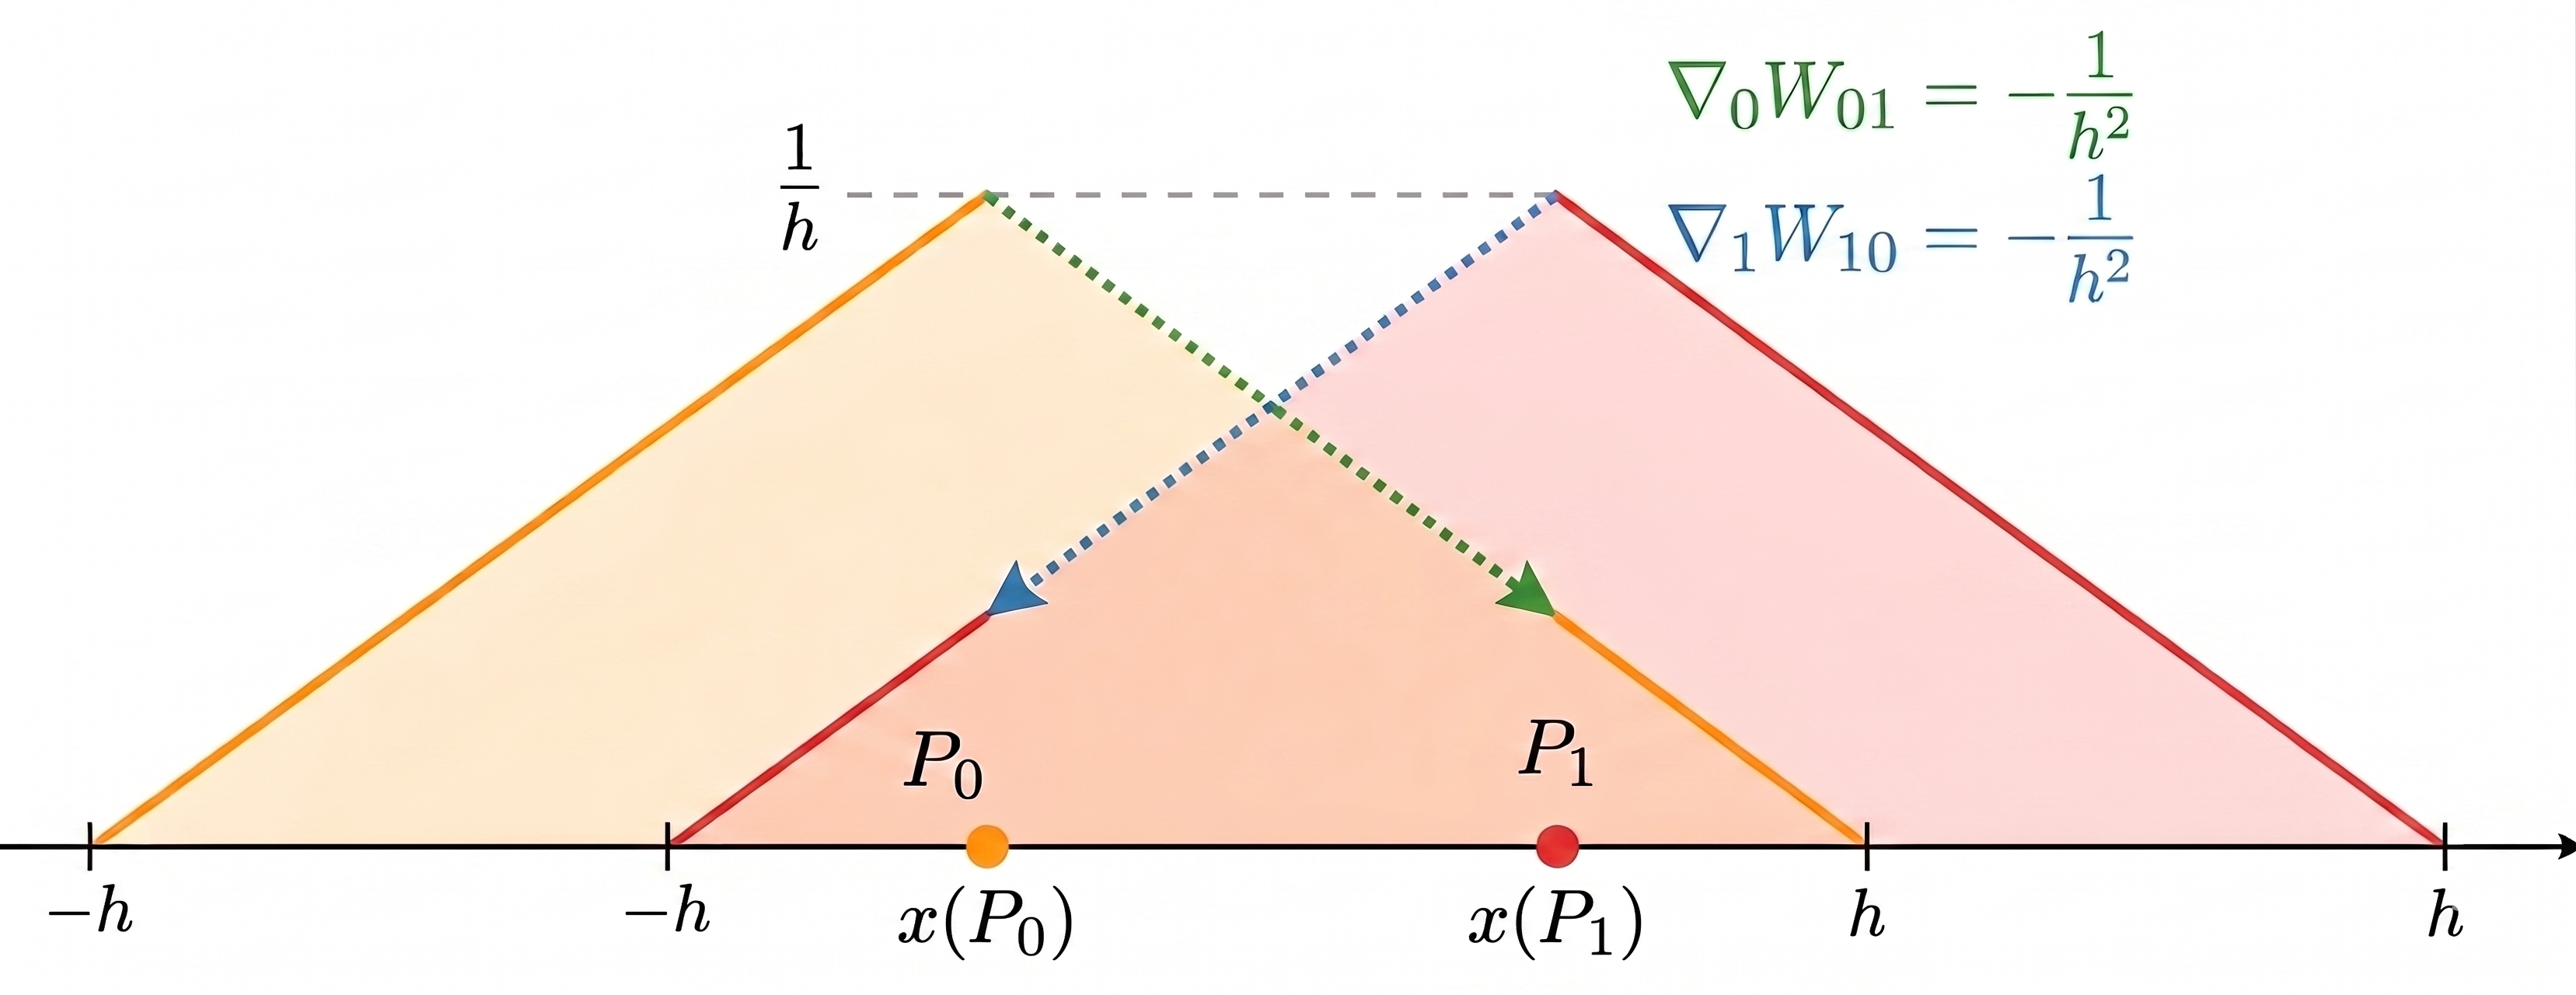
\includegraphics[width=0.9\textwidth]{chapters/cap4_metod/img/kernel_esquema.png}
    \caption{Esquema geométrico del kernel triangular y la dirección de interacción entre partículas.}
    \label{fig:kernel_esquema}
\end{figure}

Para visualizar este comportamiento de forma más gráfica, podemos remitirnos a la figura \ref{fig:kernel_esquema}. El hecho de que el valor final de $\alpha$ sea positivo obedece a una convención física fundamental, la cual implica que siempre evaluamos la derivada del kernel desde el punto de vista de la partícula $j$ hacia la partícula $k$, y nunca a la inversa. Al incorporar el operador $\nabla_j$, garantizamos que la derivada direccional sea negativa, lo que a su vez hace que la sumatoria $V_{jk}$ sea consistentemente negativa y, al multiplicarse por el signo de la ecuación, el término final $\alpha$ resulte positivo. 

Físicamente, este formalismo tiene total sentido dentro de la hidrodinámica de partículas suavizadas (SPH). Si una partícula penetra en el radio de interacción $h$ de su vecina, la geometría del kernel genera una fuerza de repulsión que cada vez debe ser más fuerte mientras más se junten las partículas, por eso un fluido se comprime hasta un límite. Si por el contrario el término $\alpha$ fuera negativo, estaríamos ante una fuerza de atracción, lo cual es inviable e inestable en este contexto. Todas las propiedades del fluido emergen de esta derivada del kernel, la cual presenta un pico de interacción máxima justo en la posición de la partícula. Son estas distintas geometrías del kernel las que, en última instancia, dictarán las propiedades macroscópicas como la viscosidad.

Finalmente, incorporando estos resultados, la matriz hermítica completa $J$ que define nuestro escenario interactivo queda conformada de la siguiente manera: 

\begin{equation}
J = 
\begin{pmatrix}
0 & c \cdot v \cdot \Delta x \\
c \cdot v \cdot \Delta x & 0
\end{pmatrix}
\label{mat: J}
\end{equation}

Con la obtención de esta matriz hermítica $J$, hemos consolidado el hamiltoniano del sistema. En el siguiente capítulo, se propone la construcción de esta matriz directamente a un circuito para computadores cuánticos universales empleando el método de \textit{Matching Decomposition}.

\section{Codificación del estado físico}
\label{sec:codificacion_estado}

Una vez definido el hamiltoniano $J$, que actúa como el escenario donde están embebidas todas las relaciones espaciales y topológicas dictadas por el kernel SPH, es necesario la definición formal entre la variable de interés del fluido (la cantidad advectada $u$) y el estado del sistema cuántico. 

Para un sistema de $N=2$ partículas, el espacio de estados puede ser representado íntegramente utilizando un único qubit, el cual define un espacio de Hilbert bidimensional $\mathcal{H} \cong \mathbb{C}^2$. En este esquema, los estados ortonormales de la base computacional identifican a las partículas mismas como entidades (o contenedores) de la propiedad física. Así, definimos:
\begin{itemize}
    \item $|0\rangle$: Representa a la partícula 0 como portadora de la cantidad advectada.
    \item $|1\rangle$: Representa a la partícula 1 como portadora de la cantidad advectada.
\end{itemize}

Para introducir la magnitud de la cantidad advectada en el computador cuántico, se recurre a la técnica de codificación por amplitud, (\textit{Amplitude Encoding}). Siguiendo la analogía descrita en la sección \ref{subsec: analogía}, el valor escalar de la cantidad advectada $u_j(t)$ en la partícula $j$ se codifica directamente como la amplitud de probabilidad del estado base correspondiente. Por lo tanto, el estado global del fluido en cualquier instante $t$ se describe mediante el vector de estado:

\begin{equation}
    |\psi(t)\rangle = u_0(t)|0\rangle + u_1(t)|1\rangle
    \label{eq:estado_cuantico}
\end{equation}

La preparación es, por tanto, un \textit{amplitude encoding}. La lectura, en cambio, se hace en la base computacional, dando como resultado que los \textit{shots} estiman las poblaciones $P_j = \rho_{jj}$. En este trabajo se identifica el escalar SPH con esas poblaciones, $u_j(t) \leftrightarrow P_j(t)$, que es la cantidad que se compara con la ecuación~\eqref{eq:sph_advection_discrete} en el capítulo~\ref{cap:resultados}.

Bajo esta formulación, el escenario espacial (la distancia entre las partículas y la fuerza de su interacción) queda dictado por el hamiltoniano. El vector de estado $|\psi(t)\rangle$ se limita a describir cómo fluye y se distribuye la cantidad advectada entre las partículas.

La normalización $\langle\psi|\psi\rangle = 1$ (o $\mathrm{Tr}\,\rho = 1$ en el caso abierto) es un postulado cuántico; no es el mismo enunciado que la conservación de masa del dímero clásico $u_0 + u_1$. En este experimento el escalar SPH se identifica con la población, $u_j^{\text{(leída)}} := P_j = \rho_{jj}$, y esa es la curva que se compara con \eqref{eq:sph_advection_discrete} en el capítulo~\ref{cap:resultados}. No se aplica $\sqrt{P_j}$ ni tomografía de amplitudes. En el circuito abierto el estado es, en general, mixto: no hay una única amplitud compleja que recuperar. El rango ficticio $u \in [0,1]$ hace legítima esa identificación en $N=2$; para magnitudes físicas con otra escala haría falta un factor clásico de normalización \textbf{antes} del \textit{encoding}, y la lectura seguiría siendo $P_j$, no $\sqrt{P_j}$.

Para el caso de estudio de este trabajo, establecemos como condición inicial que el 100\% de la cantidad advectada se encuentra concentrada en la partícula 0 en el instante $t=0$. En términos del vector de estado, esta condición se expresa como:

\begin{equation}
    |\psi(0)\rangle = 1|0\rangle + 0|1\rangle = |0\rangle
    \label{eq:condicion_inicial}
\end{equation}

Con el estado inicial definido y el hamiltoniano $J$ construido (\ref{mat: J}), la evolución analítica del sistema se rige por la aplicación del operador de evolución temporal unitaria $\hat{U}(t) = e^{-i J t}$. Las puertas universales para la ejecución de este operador $\hat{U}$ y su análisis se realiza en el siguiente capítulo.


